\documentclass[oneside]{unilasalle}

\usepackage[T1]{fontenc}
\usepackage{float}
\usepackage[latin1]{inputenc}
\usepackage{latexsym}
\usepackage{psfrag}
\usepackage{amssymb}
\usepackage{subfig}

\usepackage{url}
\usepackage{listings}
\lstset{
  basicstyle  = \footnotesize\ttfamily,
  stringstyle = \ttfamily,
  numberstyle = \scriptsize\ttfamily
}




%%%%%%

%
% Informacoes gerais => tirado do exemplo-tc.tex do Vinicius Mingot
%
\title{Monitoramento de Recursos em Ambientes de Grade}

\author{Lemos}{Daniel da Trindade}

\advisor[Profa.~DSc.]{Mangan}{Patr�cia Kayser Vargas}

% a data deve ser a da defesa; se n�o especificada, s�o gerados
% m�s e ano correntes
%\date{novembro}{2006}

% o nome do curso pode ser redefinido
\course{Ci�ncia da Computa��o}

%
% palavras-chave
% iniciar todas com letras min�sculas, exceto no caso de abreviaturas
%
\keyword{computa��o em grade}
\keyword{monitoramento}
\keyword{{\it Web services}}


%%%%%%

\begin{document}
%	%------------------------------------------------------------------------------------------------
% \simb[entrada na lista de s�mbolos]{s�mbolo}:
%   Escreve o simbolo no texto e uma entrada na Lista de S�mbolos.
%   Se o par�metro opcional e omitido, usa-se o par�metro obrigat�rio.
%------------------------------------------------------------------------------------------------
\newcommand{\simb}[2][]{%
  \ifthenelse{\equal{#1}{}}
    {\addcontentsline{los}{simbolo}{\ensuremath{#2}}}
    {\addcontentsline{los}{simbolo}{#1}}
  \ensuremath{#2}
}

\makeatletter
%------------------------------------------------------------------------------------------------
% \listadesimbolos: comando que imprime a lista de simbolos
%------------------------------------------------------------------------------------------------
\newcommand{\listadesimbolos}{
  \pretextualchapter{Lista de S�mbolos}
  {\setlength{\parindent}{0cm}
   \@starttoc{los}}}

\newcommand\listabbrname{Lista de S\'imbolos e Abreviaturas}
\newcommand\listofabbreviations{%
    \chapter*{\listabbrname
      \@mkboth{\MakeUppercase\listabbrname\space\draftdate}%
              {\MakeUppercase\listabbrname\space\draftdate}}%
     % \addcontentsline{toc}{chapter}{\MakeUppercase\listabbrname}%
    \@starttoc{lob}%
    }
\newcommand\abbrev[2]{%
                                        \def\({$}%
                                        \def\){$}%
      \addcontentsline{lob}{section}{%
                                                                \rm%
                        \protect\parbox[t]{.2\textwidth}{\bf #1}%
                   \hspace{0.025\textwidth}%
                   \protect\parbox[t]{.6\textwidth}{#2}%
        \vspace{2mm}\hspace{.1\textwidth}}%
      }

%------------------------------------------------------------------------------------------------
% como a entrada ser� impressa
\newcommand\l@simbolo[2]{\par #1, p.\thinspace#2}
		% pkvm %
	
%
% inicio do documento
%

% capa
\maketoppage

% folha de rosto
%\maketitle

\thetitlepage
\makeappage

% dedicatoria
%\clearpage
%\begin{flushright}
%\mbox{}\vfill
%{\sffamily\itshape
%``If I have seen farther than others,\\
%it is because I stood on the shoulders of giants.''\\}
%--- \textsc{Sir~Isaac Newton}
%\end{flushright}

% agradecimentos
\chapter*{Agradecimentos}

\begin{itemize}
	\item Nada se consegue sozinho, a família é a nossa base para tudo. Obrigado pai, mãe, tios, tias, irmã e todos os outros que, por algum motivo, vieram juntar-se a minha família.
	\item Aos amigos de faculdade em especial para Cristiane Ávila, Taís Américo Almeida e Wagner Nobres que, direta ou indiretamente, contribuíram para conclusão deste trabalho.
	\item Aos demais amigos que apoiaram e confiaram no meu potencial me estimulando e ajudando.
	\item Aos professores que me acompanharam e auxiliaram nesta longa caminhada, em especial a professora Patrícia Kayser, minha orientadora, que me ajudou em toda confecção deste trabalho.
	\item Aos membros do grupo do projeto GRAND que tive contato em busca de auxílio nas dúvidas encontradas.
	\item A Márcia Barbosa Abreu pela paciência, compreensão e apoio nos momentos complicados.
	\item E, principalmente a Deus, pois sem ele, nada disso poderia existir.
\end{itemize}

Muito obrigado!

\begin{abstract}
O processamento distribuído, através das Grades computacionais, conta com uma grande infra-estrutura de redes. Esta infra-estrutura pode ser empregada em compartilhamento de programas, dados e serviços. Para gerenciar essa diversidade de recursos destacam-se os Sistemas Gerenciadores de Recursos (RMS), esses sistemas têm por função gerenciar de forma cooperativa e transparente os recursos geograficamente distribuídos considerando-os como pertencentes a um único computador. Neste contexto apresenta-se o protótipo AppMan baseado no modelo GRAND ({\bf G}rand {\bf R}obust {\bf A}pplicatio{\bf n} {\bf D}eployment). Esse protótipo não implementa por completo o que sugere o modelo. Dentre as características não implementadas, cita-se a integração com diferentes RMS. Através de estudos encontrou-se a Implementação DRMMA ({\bf D}istribuited {\bf R}esource {\bf M}anagement {\bf A}pplication {\bf A}PI) que visa integrar diferentes RMS. Este trabalho demonstra a viabilidade da integração do protótipo AppMan com o RMS PBS através da DRMAA. A versão da DRMAA usada foi o pacote na linguagem Java que é a mesma linguagem do protótipo. Com a integração, foi possível submeter aplicações com um número de tarefas do que na implementação anterior. Os testes comprovaram que, apesar da necessidade de inúmeras melhorias no protótipo, a integração é possível com pouco intrusão no código atual. A versão da DRMAA usada foi o pacote na linguagem Java que é a mesma linguagem do protótipo.
\end{abstract}

\begin{englishabstract}{Integration of the AppMan Application Management for the Grid Environment with the Resource Management Systems PBS}{Grid Computing, Resource Management}
Distributed Processing in Computational Grids can use a large  networks infrastructure. This infrastructure can be used in sharing of programs, data, and services. We can use a Resource Management System (RMS) to manage this diversity of resources.  Such a system can manage in a cooperative and transparent way the resources geographically distributed considering them as belonging to a single computer. In this context, there is a prototype model called AppMan based on the GRAND ({\bf G}rand {\bf R}obust {\bf A}pplicatio{\bf n} {\bf D}eployment) model. This prototype doesn't fully implement the GRAND model. The GRAND model, missing specifically the integration with different RMS. Through studies we found the DRMAA ({\bf D}istribuited {\bf R}esource {\bf M}anagement {\bf A}pplication {\bf A}PI) implementation which aims to integrate different RMS. This work demonstrates the feasibility of integrating the prototype AppMan with the PBS RMS through DRMAA. Tests have shown that, despite the need for numerous improvements in the prototype, integration is possible with little intrusion in the current code. The DRMAA version used was a Java language API that is the same language of the prototype.
\end{englishabstract}		% pkvm %
	%dtl%\begin{resumo}
%pkvm%
\begin{abstract}
Em um ambiente de computa��o em grade, ...  Assim, este trabalho busca um modelo de monitoramento de recursos de
hardware e software, que contemple as quest�es de escalabilidade e
heterogeneidade,para ambientes de grade. 
Um prot�tipo foi implementado ... . As avalia��es mostraram ....






%O Sistema Operacional atendido pelo prot�tipo � Windows. 
%Uma vez com o prot�tipo finalizado, foi utilizado como ambiente de teste o laborat�rio do Banrisul \abbrev{BANRISUL}{Banco %do %Estado do Rio Grande do Sul}.Os resultados da mo\-ni\-to\-ra\-��o ser�o disponibilizados no formato XML %\abbrev{XML}{\emph{eXtensible Markup Language}} para facilitar a integra��o com outras ferramentas.

%Posteriormente, deseja-se montar uma grade de teste envolvendo m�quinas do laborat�rio 24h do Unilasalle, da UFRJ %\abbrev{UFRJ}{Universidade Federal do Rio de Janeiro} e da UFLA\abbrev{UFLA}{Universidade Federal de Lavras} para teste do %sensor Linux. Os resultados da mo\-ni\-to\-ra\-��o ser�o 
%disponibilizados no formato XML \abbrev{XML}{\emph{eXtensible Markup Language}} para facilitar 
%a integra��o com outras ferramentas.
%dtl%\end{resumo}
%dtl%\begin{abstract}
\end{abstract}

% resumo na outra l�ngua
% como parametros devem ser passados o titulo e as palavras-chave
% na outra l�ngua, separadas por v�rgulas

%\selectlanguage{english}

\begin{englishabstract}{Resource Monitoring in Grid Environments}{Grid Computing, Monitoring, Web Services}
In a grid computing environment, ...
Thus, this work aims at proposing a hardware and software resource
monitoring model for grid environment, which deals with scalability
and heterogeneity issues.
A prototype was implemented ... The evaluation showed ...
\end{englishabstract}

%\selectlanguage{brazilian}

		% pkvm %
	
% sumario
\tableofcontents

% lista de abreviaturas e siglas
% o parametro deve ser a abreviatura mais longa
% => obtido do padrao do II-UFRGS (utug-l)
%%%%% aqui tem que trocar pela tua lista!
\begin{listofabbrv}{SPMD}
        \item[SMP] Symmetric Multi-Processor
        \item[NUMA] Non-Uniform Memory Access
        \item[SIMD] Single Instruction Multiple Data
        \item[SPMD] Single Program Multiple Data
        \item[ABNT] Associa��o Brasileira de Normas T�cnicas
	\item[XML] eXtensible Markup Language
\end{listofabbrv}

% lista de figuras
\listoffigures

% lista de tabelas
\listoftables

		% pkvm %

	\section*{Introdução}
\label{cap:introducao}

Atualmente o uso de redes de computadores tem aumentado exponencialmente. Muitas dessas redes são distribuídas de forma geograficamente separadas precisando de uma complexa infra-estrutura de software e hardware para gerenciá-las e conectá-las. Dentre as diversas soluções existe a grade computacional (\emph{grid computing}).

Segundo Dantas \cite{Mangan2006}, pode-se dizer, também, que representa uma forma estendida dos serviços web permitindo que recursos computacionais possam ser compartilhados.

Defini-se grades como uma plataforma computacional heterogênia distribuída geograficamente fornecendo serviços e recursos às organizações participantes da plataforma \cite{Mangan2006}.

\cite[apud]{Mangan2006} O Global Grid Forum (GGF) uma comunidade fórum com milhares de indivíduos representando mais de 400 organizações em mais de 50 países criou e documentou especificações técnicas e experiências de usuários. O GGF definiu grades computacionais como um ambiente persistente o qual abilita aplicações para integrar intrumentos, disponibilizar informações em locações difusas. Desde lá não é a única e precisa definição para o conceito de grades. \cite{Kesselman2001} Define um sistema em grade propondo um \emph{checklist} de três pontos.

\begin{enumerate}
	\item coordena recursos quais não são direcionados para um controle central.
	\item usa protocolos e interfaces padronizados, abertos para propósitos gerais
	\item oferece QoS (qualidade de serviço) não triviais tais como: autenticação, escalonamnto de tarefas, disponibilidade.
\end{enumerate}

Uma definição formal do que um sistema em grade pode prover foi definido em \cite{Mangan2006}. Focando na sua semântica, mostrando que grades não são apenas uma modificação de um sistema distribuído convencional. Podem apresentar recursos heterogênicos como sensores e detectores e não apenas nós computacionais. Abaixo uma lista de aspectos que evidenciam uma grade computacional \cite{Cirne2002}

\begin{itemize}
	\item heterogeneidade
	\item alta dispersão geográfica
	\item compartilhamento ( não pode ser dedicado a uma única aplicação )
	\item múltiplos domínios administrativos ( recursos de várias instituições )
	\item controle distribuído 
\end{itemize}

A grade deve estar preparada para lidar com todo o dinamismo e variabilidade, procurando obter a melhor performance possível adaptando-se ao cenário no momento.

Devido à grande escala, ampla distribuição e existência de múltiplos domínios administrativos, a construção de um escalonador de recursos para grades é impossível, até porque, convencer os administradores dos recursos que compõem a grade abrirem mão do controle dos seus recursos não é nada fácil. Escalonadores têm como características receber solicitações de vários usuários, arbitrando, portanto, entre os usuários, o uso dos recursos controlados. 		% Inclus�o da Introdu��o
	\chapter{Monitoramento em Grade}
\label{cap:Monitoramento_Grade}

...


Segundo Jain \cite{jain91} um monitor � uma ferramenta utilizada para ...


As informa��es de monitoramento de hardware e software devem ser coletadas m�quina a m�quina, mas normalmente s�o
centralizadas nas redes locais ou {\it clusters}. 


\section{\label{sec_Trab_Relacionados}Trabalhos Relacionados}

 ...

\subsection{\label{subsec_Ganglia}Ganglia}

...

\subsection{\label{subsec_Condor_Hawkeye}Condor e Hawkeye}

...


\subsection{\label{sec_globus_WebMds}Globus e WebMDS}



\subsection{\label{subsec_Grads_NWS}GrADS e NWS}

...


\section{\label{sec_analise}An�lise}

...	% Inclus�o do Capitulo de Monitoramento
	\section{Modelo Proposto}
\label{cap:modelo proposto}


O protótipo AppMan é uma implementação simplificada do GRAND. Ele usa a ferramenta JavaCC para implementar o {\it parsing} e interpretação da GRID-ADL. A figura 2 representa um possível cenário do AppMan sendo executado sobre um ambiente de grade.

O passo 1 da figura representa o usuário submetendo um arquivo de descrição na linguagem GRID-ADL. Esse arquivo é analisado e o grafo de aplicação é feito na memória. Um algoritmo é executado e os sub-DAGs do grafo de aplicação é obtido. O {\it Application Manager} (AM) é inicializado. Então o AM instancia {\it Submission Managers} (SM) no passo 2 e distribui alguns subgrafos para os SMs. Os arquivos de entrada e os executávies são obtidos através de um {\it web server} (passo 3). Na sua atual implementação, AppMan necessita que o usuário indique as máquinas onde os SMs irão ser executados. Com essa simplificação um novo SM é instanciado para cada aplicação em cada máquina especificada. Após a criação dos SMs, o AM determina subgrafos para cada SM. Os SMs informam para o AM o progresso das tarefas. Cada SM, independentemente, verifica a lista das máquinas disponíveis e escolhe aleatoriamente um nó para executar a tarefa. Antes de iniciar a execução de uma tarefa, AppMan transfere todos arquivos de entradas especificados na descrição GRID-ADL para um diretório temporário no nodo remoto onde a tarefa será executada. O arquivo de transferência é executado automaticamente. Então, cada SM recupera a informação atualizada através do serviço de informação do EXEHDA sobre os nodos avaliados. Cada SM escolhe onde irá executar estas tarefas aleatoriamente. Imediatamento um TM é instanciado criando a tarefa remota e monitorando até que a execução da tarefa termine (passo 4).

\begin{figure}[h]
\center
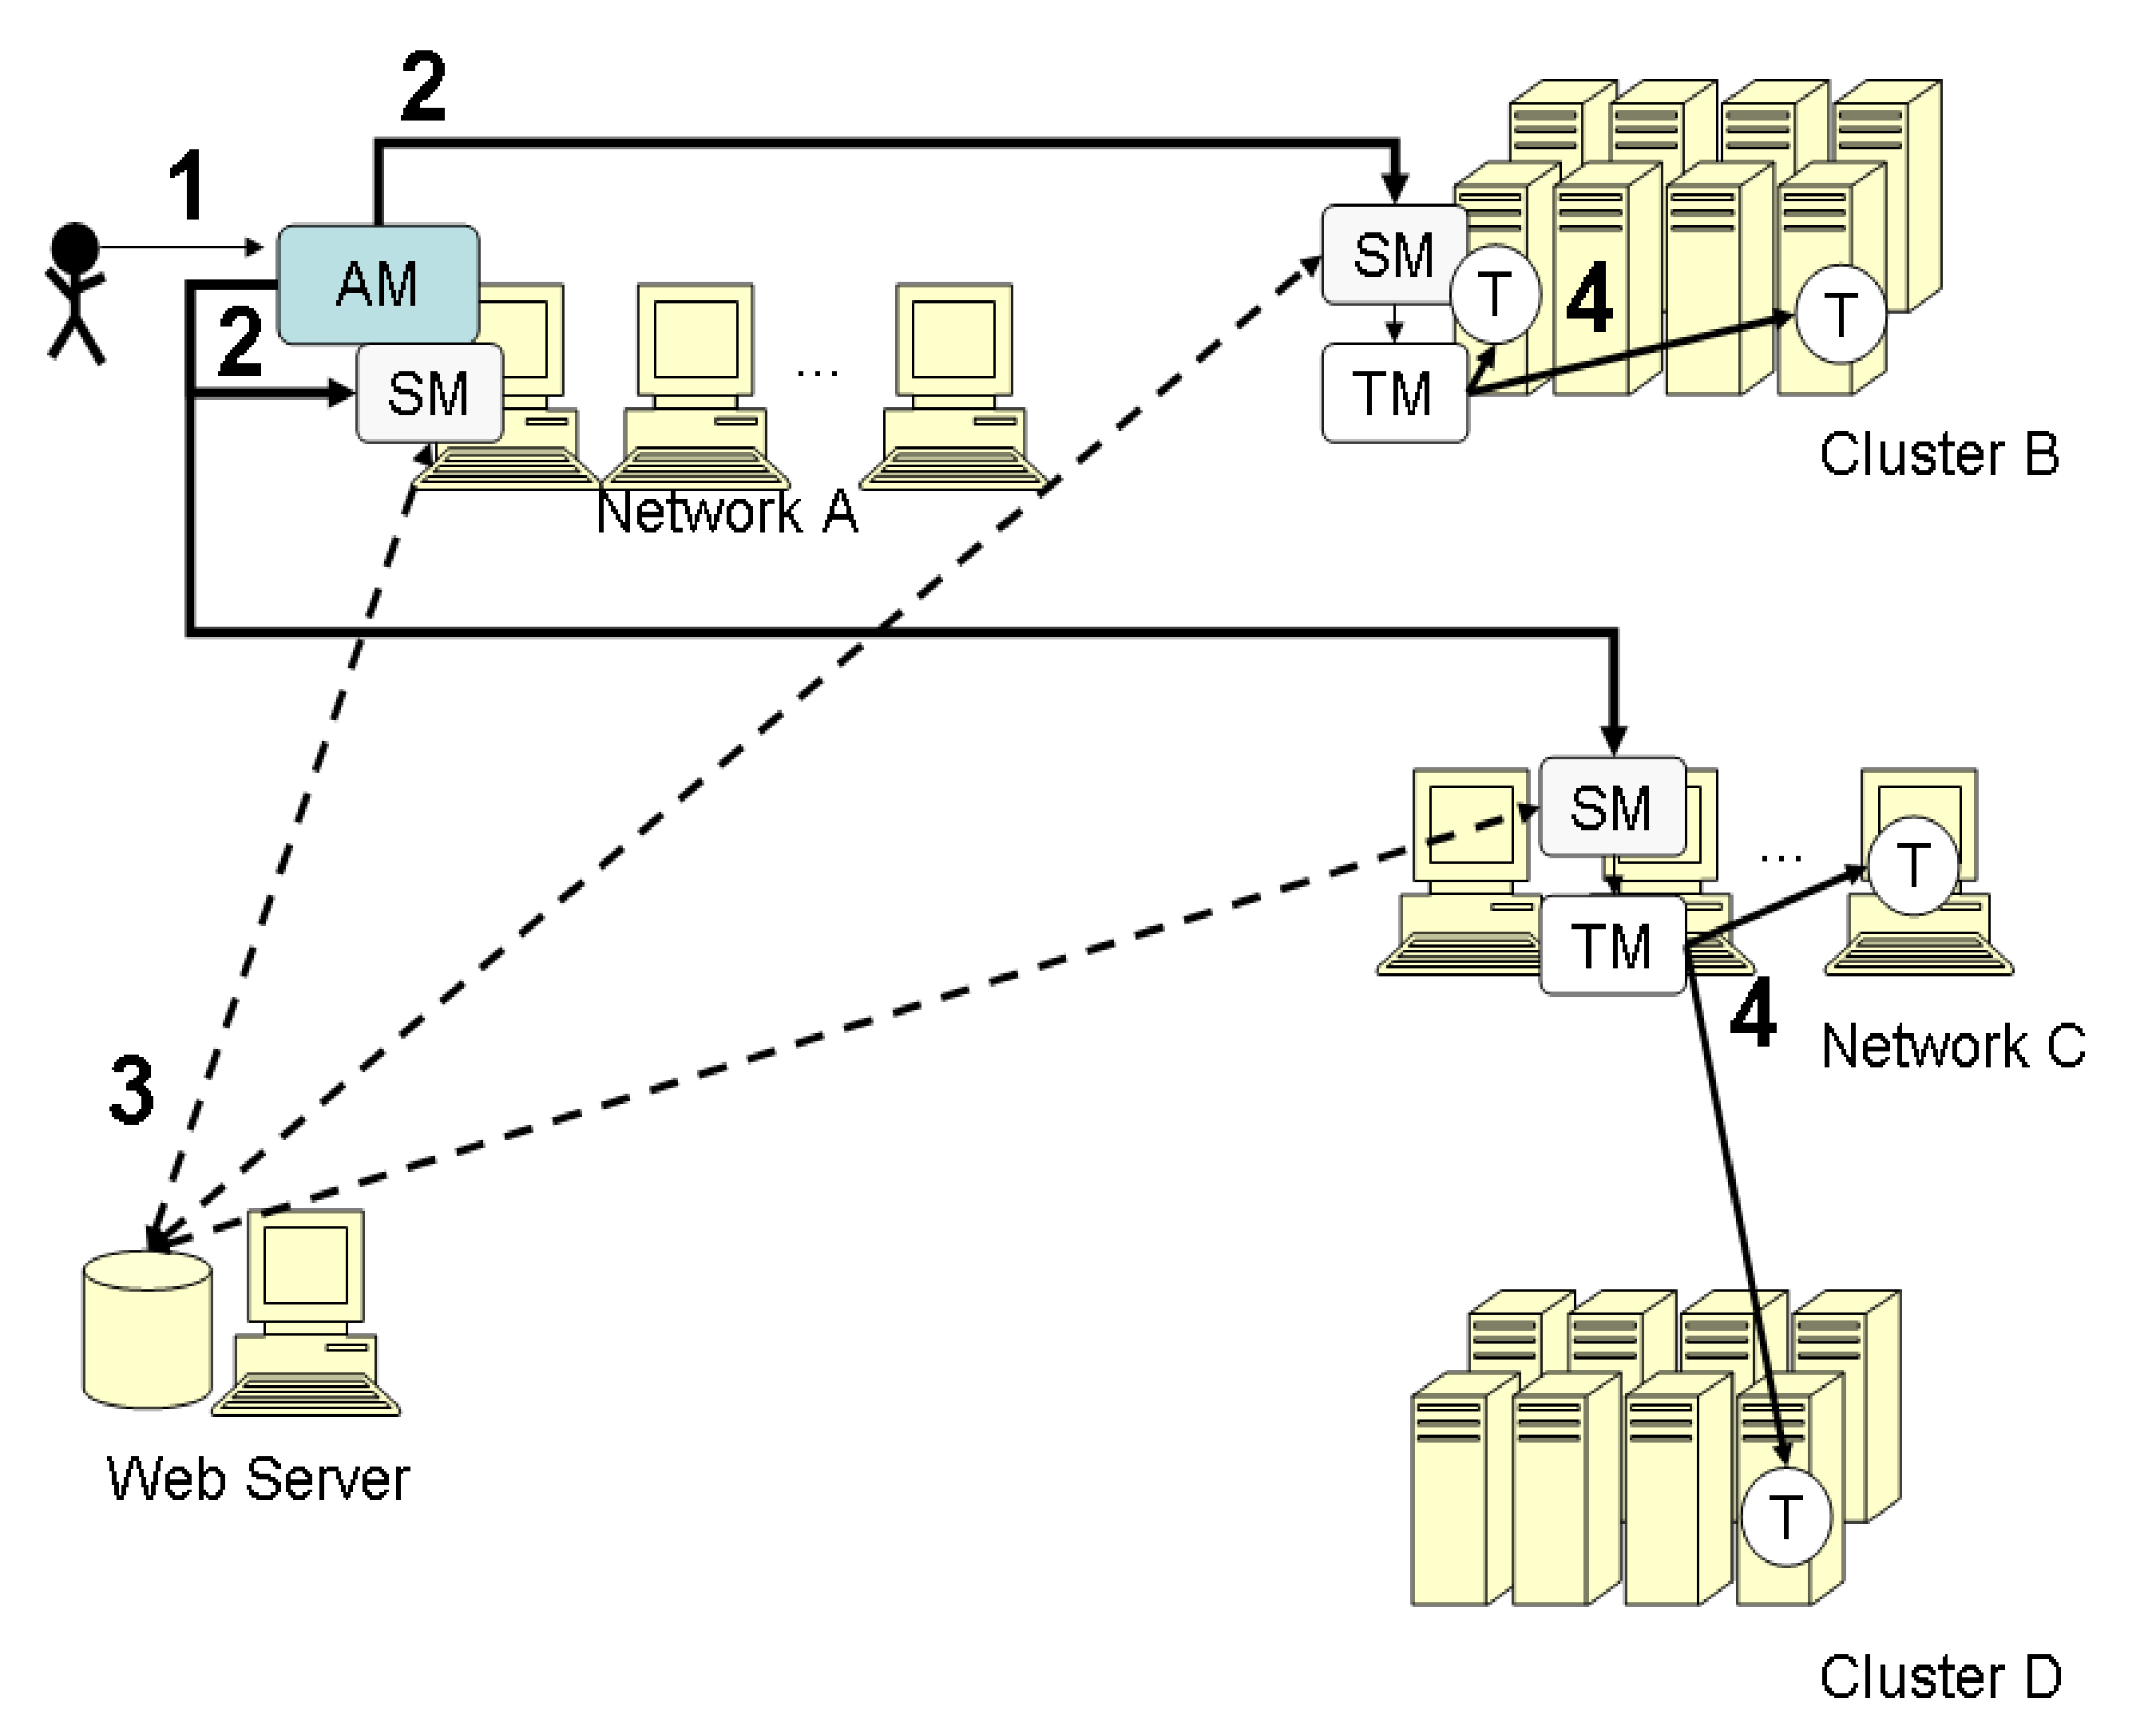
\includegraphics[scale=.2]{img/AppMan.eps}
\label{AppMan}
\caption{AppMan executando principais passos}
\end{figure}

Como sugere o modelo GRAND, o AppMan não possibilita o escalonamento através de outros RMS. É necessário que o EXEHDA e o AppMan estejam presentes em todos nós da grade. Integrar o AppMan com outros RMS possibilitará uma maior escalabilidade da grade e também possibilitará uma aproximação do AppMan ao que sugere o modelo GRAND. Os nodo principais de cada {\it cluster} que compõem a base possuem nodos abaixo delas. O AppMan espera um serviço de compartilhamento de arquivo entre os nodos e base. Isto é, mais uma característica que impossibilita o uso de outros RMSs com o AppMan

Uma especificação {\it Distributed Resource Management Application} \cite{Rajic2002} desenvolvida pelo OGF, tem por objetivo abstrair as diferenças dos RMS e fornecer uma API visando facilitar a integração de aplicações. O escopo da DRMAA é limitada a submissão, monitoramento e controle das tarefas além de retornar status de conclusão de uma tarefa. Inicialmente implementada na linguagem C, atualmente possui uma implementação na linguagem Java, apesar de oferecer suporte apenas para o {\it Sun Grid Engine} \cite{Templeton}.
Inúmeros relatórios técnicos N1™ Grid Engine \cite{Templeton2006}, GridWay \cite{Herrera2007}, Condor \cite{Troeger2007} e PBS \cite{Ciesnik2007} de implementações com a DRMAA concluem possitivamente para as implementações. Não havendo a necessidade de grande inteferência no código dos RMSs citados.

Em um primeiro estudo da documentação do AppMan pode-se notar duas principais classes, {\it TaskManager} (Figura 3) e {\it SubmissionManager}. A classe {\it SubmissionManager} implementa os métodos da {\it Interface SubmissionManagerRemote} a qual possui os métodos que recuperam informações das tarefas executadas remotamente e o metódo da geração do grafo da aplicação. A classe {\it TaskManager } implementa a interface {\it TaskManagerRemote} contendo os métodos tais como os que adicionam tarefas na lista de execução remota.

\begin{figure}[h]
\center
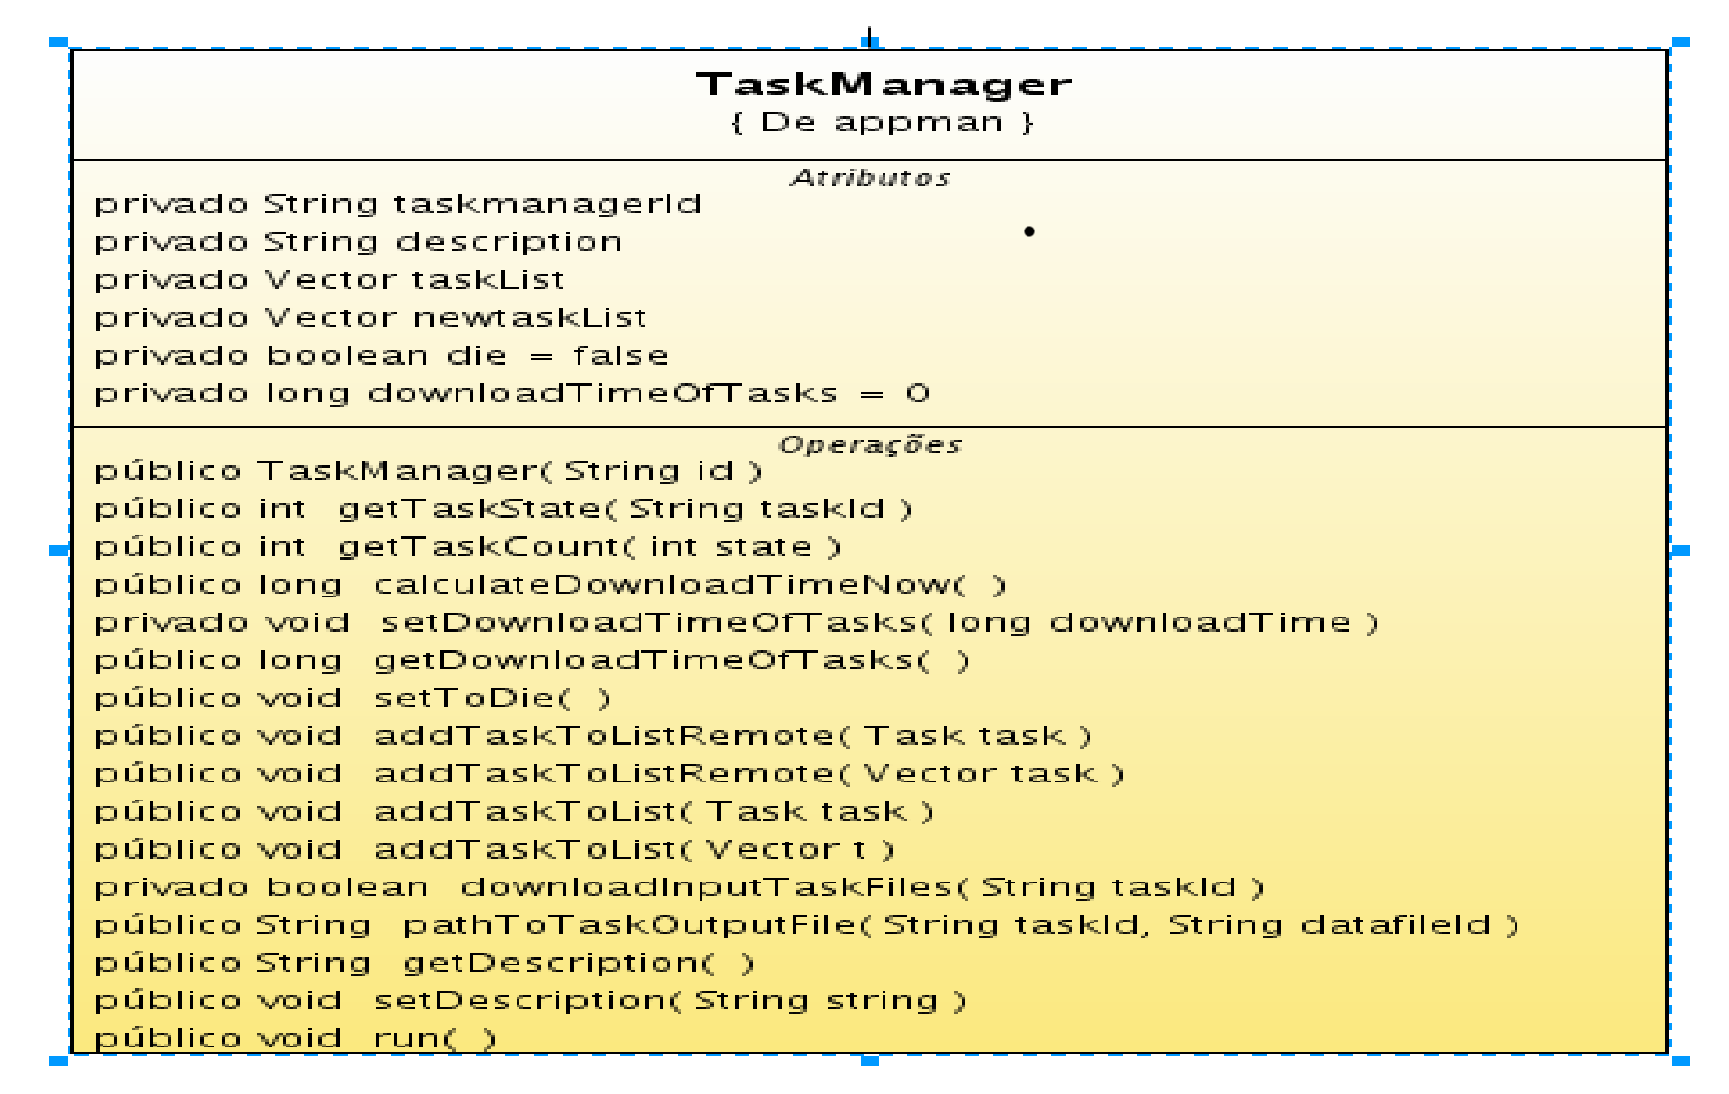
\includegraphics[scale=.4]{img/TaskManager.eps}
\label{TaskManager}
\caption{Classe TaskManager}
\end{figure}

Baseado no que foi analisado até o momento da confecção deste artigo, notou-se a necessidade de alteração na {\it Interface TaskManagerRemote} onde necessitará ser adicionado métodos que implementarão as especificações da DRMAA. Essa seria a melhor forma de implementação com a mínima interferência no código atual. Principalmente por existirem trabalhos nessa área {\it quero citar o tc do Wagner aqui}.

A presente proposta de pesquisa proporcionará uma maior dispersão geográfica para o AppMan pois, novos domínios adimistrativos (instituições) poderão fazer parte da grade em que se encontra. Contribuiria, também, para o AppMan ficar próximo de atingir o que propõem o modelo GRAND resolvendo o problema da necessidade do EXEHDA/AppMan estarem presentes em todos nós da grade. 

A figura 4 mostra como deverá ficar o funcionamento do AppMan após a realização do trabalho proposto. Os TMs nos nós locais contatam RMSs remotos dispachando as tarefas para esses RMSs.

\begin{figure}[h]
\center
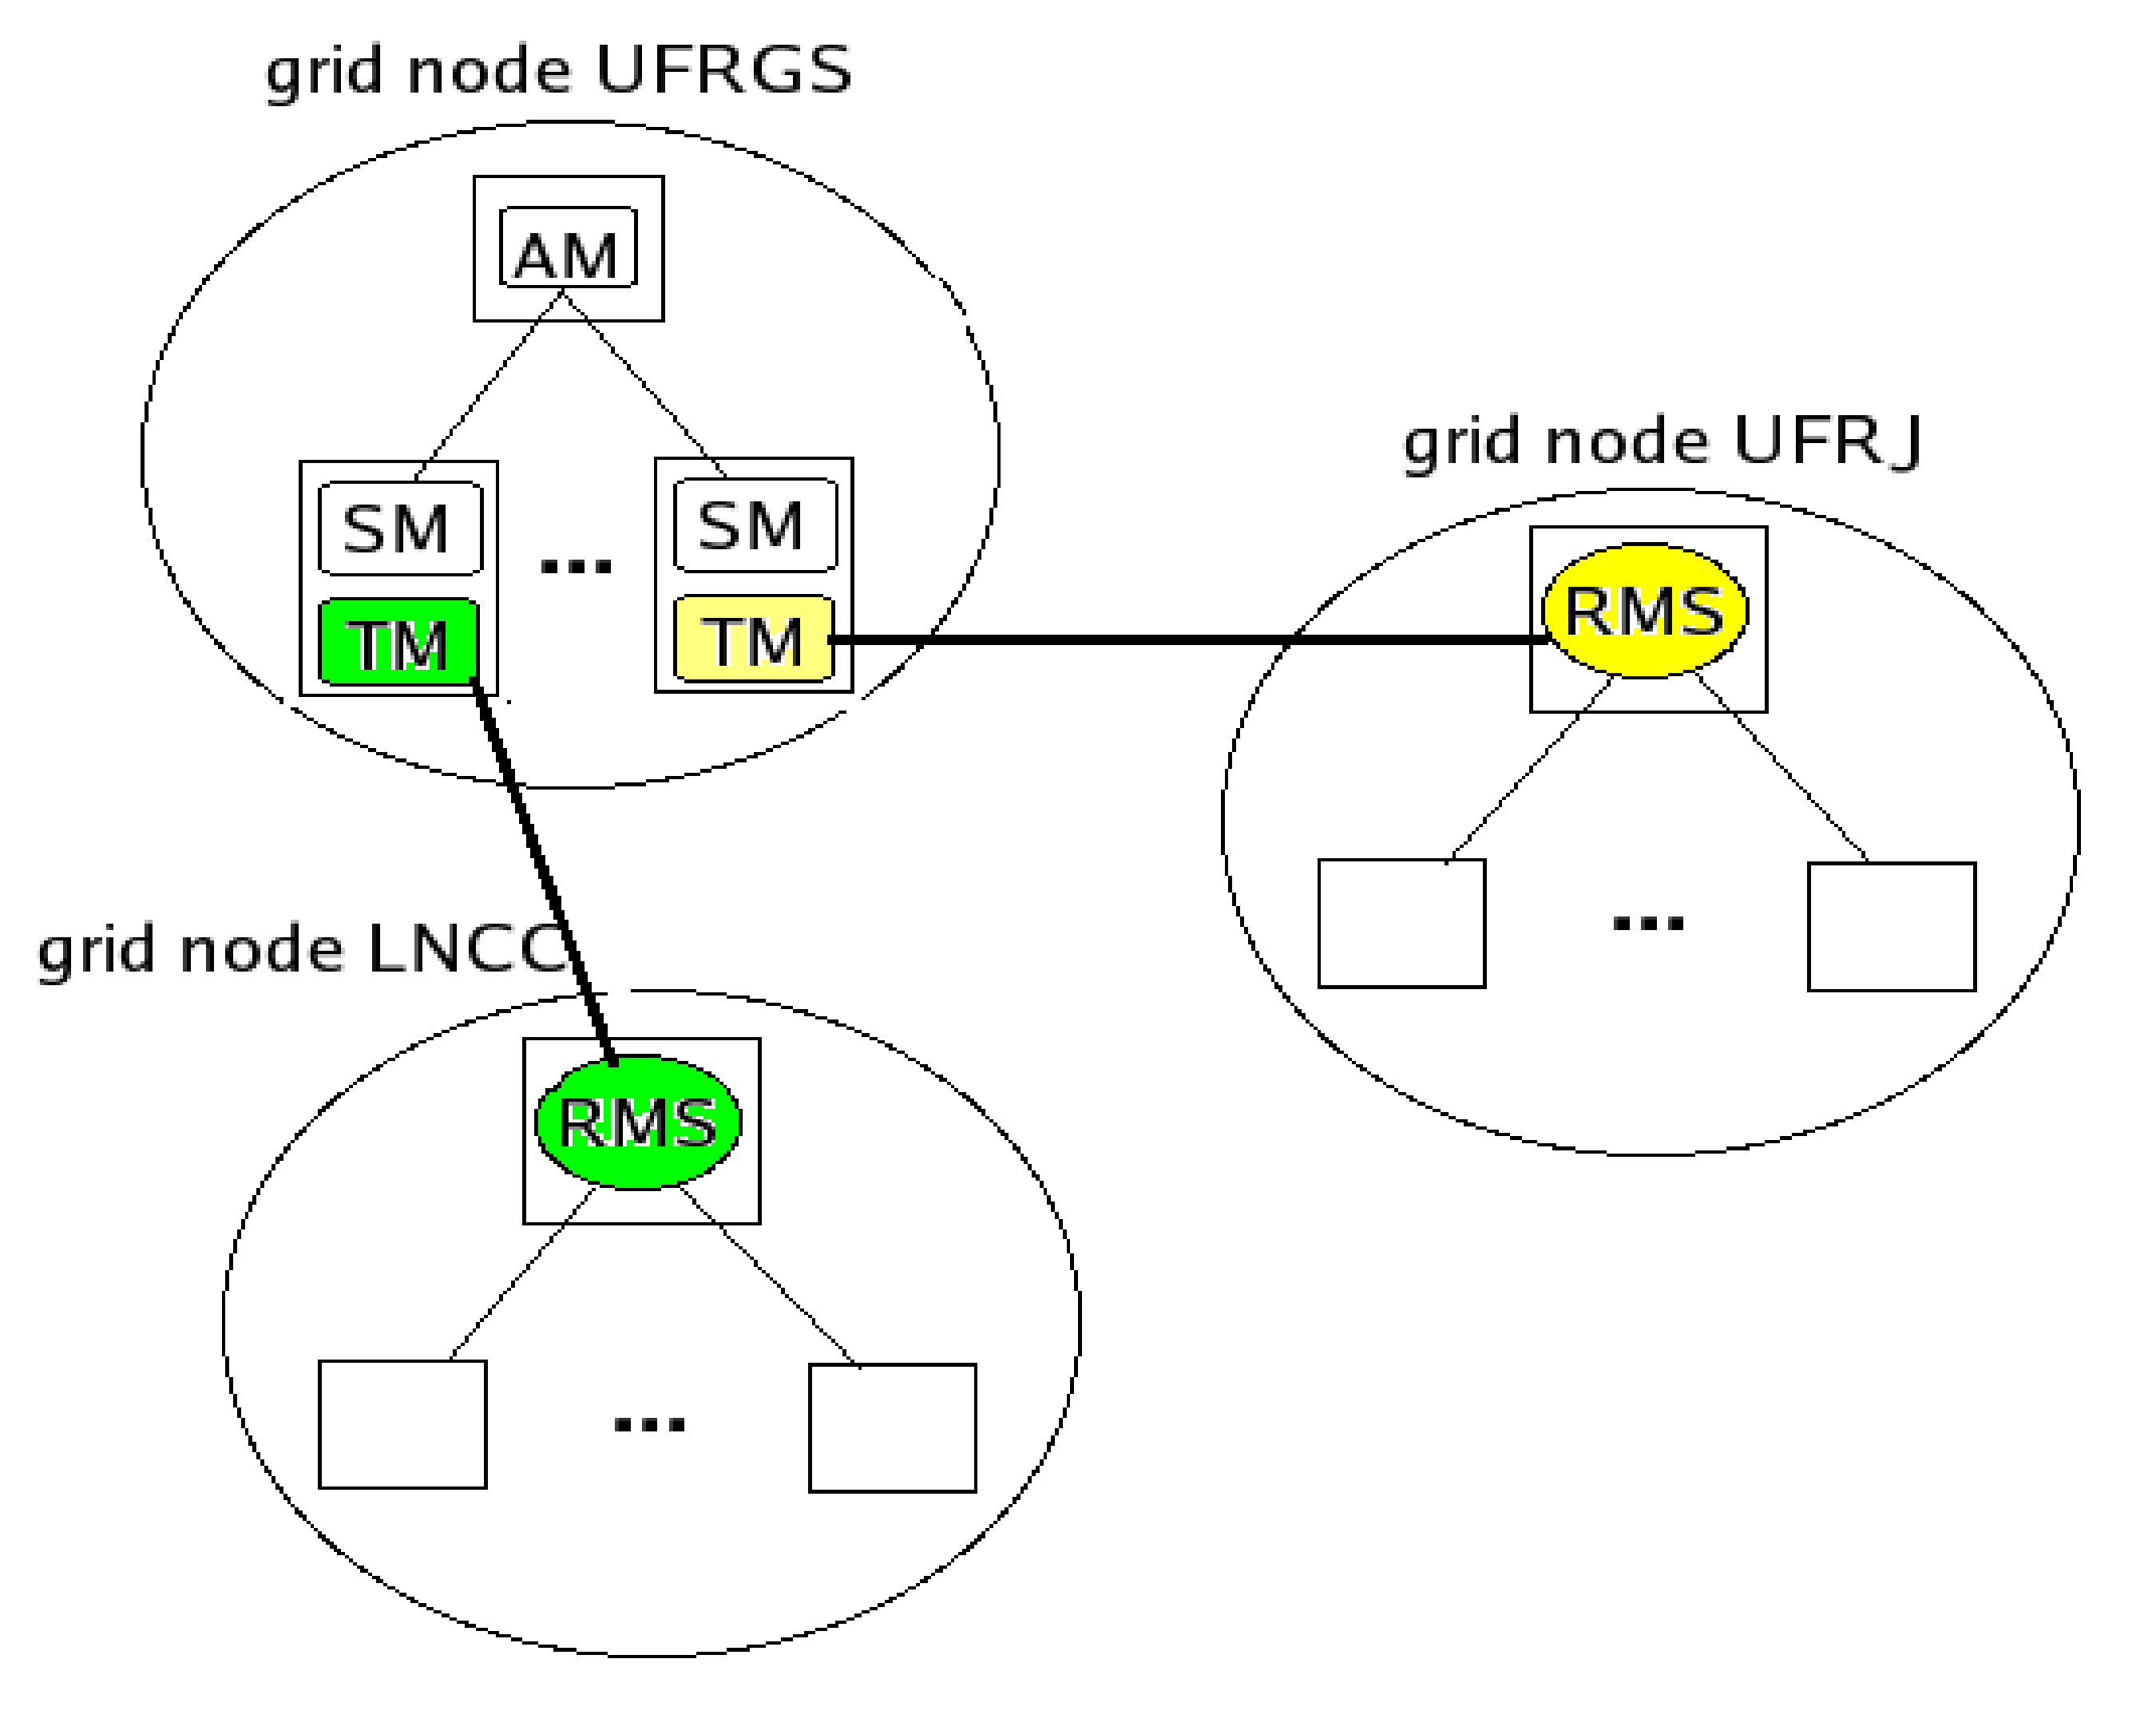
\includegraphics[scale=.2]{img/AppManRMS.eps}
\label{AppManRMS}
\caption{AppMan executando em um cenário com TMs comunicando com RMS}
\end{figure}

O modelo proposto para o TCC consiste em avaliar se a especificação DRMAA atende as necessidades do AppMan bem como realizar a integração do AppMan ao menos com um RMS.
		% Inclus�o do Capitulo de Modelo
	\chapter{Dados Experimentais}
\label{cap:Dados_Experimentais}

Este cap�tulo apresenta os resultados dos ...


Para a m�dia foi calculada a m�dia aritm�tica simples e para o desvio foi calculado atrav�s da f�rmula do desvio padr�o (n�o-polarizado ou n-1) escrita assim:

\begin{center}
\begin{math}
\sqrt{ \frac{n\sum x^{2} - (\sum x)^{2}}{n(n-1)}}
\end{math}
\end{center}



\section{\label{sec_Intrusao_Maquina}Intrus�o na M�quina}


A Tabela \ref{tab:intrusao_maquina} mostra o ...


\begin{table} [hbtp]
\begin{center}
\caption{Intrus�o nas M�quinas}
\label{tab:intrusao_maquina}
%\begin{footnotesize}
\begin{scriptsize}
\begin{tabular}{l|l|l|l|l|l}
	\hline
		{\bf Equipamento} & \multicolumn{3}{c|}{\bf Ocupa��o CPU} &  {\bf Mem�ria} &  {\bf Tam. Arq. Gerado}\\
				  &	M�x	&  M�d	& 	Desvio	  & 	  	   & 			    \\
	\hline
		Equip 1		  &  50 \%	& 24 \%	 & 	19 \%	  &   3 MB	   & 	17 Kbytes	    \\ \hline
		Equip 10	  &  49	\%	& 23 \%	 & 	16 \%	  &   5 MB	   & 	16 Kbytes	    \\ \hline \hline
		\bf{M�dia}	  &  49,7 \%	& 23,2 \%&	17,5 \%	  &  5,6 MB	   &	16,2 Kbytes	    \\ \hline
		\bf{Desvio Padr�o}&  0,48 \%	& 1,03 \%&	1,64 \%	  &  1,64 MB	   &	0,78 Kbytes	    \\ \hline



\end{tabular}
%\end{footnotesize}
\end{scriptsize}
\end{center}
\end{table}


	% Inclus�o do Capitulo de Dados Experimentais
	\section{Conclusão}
\label{cap:conclusao}

O projeto GRAND, atualmente, possui uma série de cooperações informais com várias instituições de pesquisa como, UFRGS, UFRJ, UFLA e Universidade do Porto. Além das contribuições já existentes no projeto ao qual esta pesquisa está inserida, a integração do AppMan com RMSs diferentes através da DRMAA aumentaria a perspectiva de novos domínios administrativos integrarem na grade ampliando a escalabilidade. Também possibilitaria uma quantidade maior de teste no modelo GRAND. Através desse estudo inicial, além da especificação DRMAA, vários sistemas de gerenciamento de recursos foram estudados.

Como contribuições futuras, além de integrações com demais RMSs, a solução do problema da necessidade de existir um serviço de compartilhamento de arquivos em funcionamento entre os nós da grade.
		% Inclus�o do Cap�tulo de Conclus�o
	\appendix
\addcontentsline{toc}{chapter}{Ap�ndices}
\chapter {Documento XML do Sensor Completo}
\label{anexo:xml_completo}

\begin{scriptsize}
\begin {verbatim}
  <?xml version="1.0" encoding="utf-8" ?> 
 <Computador xmlns:BMS="http://n061/bms/link">
 ...
</Computador>

\end{verbatim}
\end{scriptsize}




%=============================
\chapter{GRID-ADL ABNF}
\label{appendix:gridADL}


%% listing - decrease fonte size%%
%\lstset{
%  basicstyle  = \scriptsize\ttfamily,
%}
%%
\begin{lstlisting}
;
; The input_file non-terminal is the starting point of this grammar
<input_file> = [ <graph_definition> ]
               [ <application_requirements> ]
               <set_of_task_definition>
               [ <transient_file_definition> ]
...
\end{lstlisting}

%% listing - return to previous value %%
%\lstset{
%  basicstyle  = \footnotesize\ttfamily,
%}
%%			% Inclus�o do Cap�tulo de Anexos
	%\bibliographystyle{abnt-alf}
\bibliographystyle{apalike}
\bibliography{biblio}
		% Inclus�o da bibliografia
\end{document} 
